%----------------------------------------------------------------------------------------
%	PENDAHULUAN
%----------------------------------------------------------------------------------------
\section*{TINJAUAN PUSTAKA} % Sub Judul PENDAHULUAN
% Tuliskan isi Pendahuluan di bagian bawah ini. 
% Jika ingin menambahkan Sub-Sub Judul lainnya, silakan melihat contoh yang ada.
% Sub-sub Judul 
\subsection*{\textit{Map-reduce}}
\textit{Map-reduce} merupakan pemodelan pemograman yang digunakan untuk memproses data yang berukuran besar pada lingkungan paralel (\citeauthor{DEAN2004} \cite*{DEAN2004}). Pemodelan \textit{map-reduce} mempunyai \textit{run time system} yang menjadi salah satu kelebihan dari pemodelan ini. \textit{Run time system} dapat menangani masalah pembagian data dan penanganan kesalahan sistem. \textit{Map-reduce} memiliki dua tahap yang yaitu \textit{map} dan \textit{reduce}. \textit{Map} dan \textit{reduce} dijalankan secara terpisah namun sama-sama dilakukan secara paralel. Setiap langkah mempunyai atribut \textit{key} dan \textit{value} yang sepasang. \textit{Map} berfungsi untuk memetakan input ke dalam beberapa node dan memasangkan \textit{key} dan \textit{value} pada tiap node.  Komputer yang menjalankan tahap ini disebut \textit{mappers}. \textit{Reduce} berfungsi untuk menyatukan hasil dari \textit{map} dengan melihat \textit{key} yang diberikan pada tahap \textit{map}. \textit{Reduce} juga akan memblokir proses sampai data dari \textit{map} sudah semua ditransfer (\citeauthor{TAYLOR2010} \cite*{TAYLOR2010}). Komputer yang menjalankan tahap ini disebut \textit{reducers}.

% Sub-sub Judul 
\subsection*{\textit{K-mers Frequency}}
K-mers frequency merupakan frekuensi untuk menghitung banyaknya kemunculan dari subsequence yang mungkin dari 4 kombinasi (A, T, G, dan C) dengan panjang k pada suatu sekuen DNA. Setiap kombinasi akan dihitung sesuai dengan kombinasi dari sekuen DNA sebanyak k. Subsequence yang akan dihitung menggunakan nilai k sama dengan 3 akan menghasilkan pola ciri sebesar 43 atau 64 base pair. Pola ciri yang didapatkan adalah {AAA, AAC, AAT, AAG, ACA, ACC, ACT, ACG, ATA, ATC, ATT, ATG, AGA, AGC, AGT, AGG, CAA, CAC, CAT, CAG, CCA, CCC, CCT, CCG, CTA, CTC, CTT, CTG, CGA, CGC, CGT, CGG, TAA, TAC, TAT, TAG, TCA, TCC, TCT, TCG, TTA, TTC, TTT, TTG, TGA, TGC, TGT, TGG, GAA, GAC, GAT, GAG, GCA, GCC, GCT, GCG, GTA, GTC, GTT, GTG, GGA, GGC, GGT, GGG}. Ilustrasi perhitungan k-mers frequency  pada sekuen DNA dapat dilihat pada Gambar \ref{fig:mers}.

\begin{figure}[h!]\centering % Gunakan \begin{figure*} untuk memasukkan Gambar
	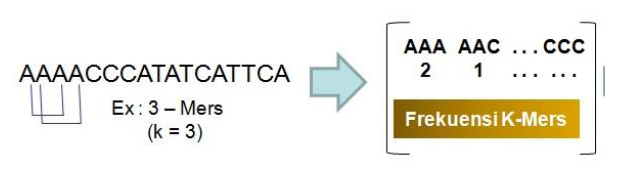
\includegraphics[width=200pt]{mers.png}
	\caption{Ilustrasi perhitungan \textit{k-mers}}
	\label{fig:mers}
\end{figure}

\subsection*{\textit{Single Link}}
Dalam analisis kluster pada dasarnya akan dilakukan pengelompokan secara alami terhadap sekelompok objek, dengan melakukan perbandingan terhadap masing-masing objek yang memiliki tingkat kesamaan atau jarak. Pengelompokan adalah proses pembelajaran \textit{unsupervised} terhadap suatu \textit{pattern} untuk dijadikan beberapa kelompok berdasarkan kemiripan (\citeauthor{JAIN1999} \cite*{JAIN1999}). Kluster adalah koleksi dari \textit{record} yang mirip dan tidak mirip dengan \textit{record} dari kluster lain. Pengelompokan  berbeda dengan klasifikasi, dalam hal ini tidak ada variabel target untuk dikelompokkan. Pengelompokan tidak mengklasifikasikan, meramalkan atau memprediksi nilai dari sebuah variabel target. Algoritme pengelompokan digunakan untuk menentukan segmen keseluruhan himpunan data menjadi subgrup yang relatif sama atau kluster, dengan kesamaan record dalam kluster dimaksimumkan dan kesamaan \textit{record} di luar kluster diminimumkan (\citeauthor{LAROSE2005} \cite*{LAROSE2005}).

Pengelompokan data dengan metode \textit{single link} termasuk ke dalam metode \textit{hierarchical agglomerative clustering}. \textit{Hierarchical} melihat objek yang mirip yang nantinya akan dikelompokkan. Hasilnya dalam bentuk dendogram yang akan menampilkan gambaran antarkelompok yang terdekat. Ilustrasi dendogram dapat dilihat pada Gambar \ref{fig:dendogram}.

\begin{figure}[h!] % Gunakan \begin{figure*} untuk memasukkan Gambar
	\centering
	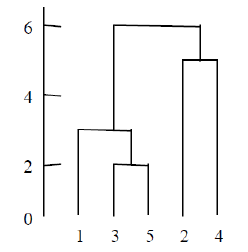
\includegraphics[width=200pt]{den.png}
	\caption{Ilustrasi dendogram pada \textit{single link}}
	\label{fig:dendogram}
\end{figure}

\textit{Single link} akan mengelompokkan objek berdasarkan jarak terdekat antaranggota. \textit{Input} dari metode \textit{single link} bisa berupa jarak atau tingkat kesamaan antara pasangan dari objek. Objek akan dikelompokkan berdasarkan jarak terdekat, dipilih nilai terkecil lalu digabungkan, dan hasilnya akan dibandingkan kembali dengan jarak pada kelompok lain.


